\section{Ablation and Comparative Analysis}
\label{sec:ablation}

\textbf{Ablation (E5).} Table~\ref{tab:ablation} removes one component at a time from SpecLoop on Dafny. Python is left out because the shared first candidate already solves about 96\% of the Python instances, so no component can change the outcome there. When SpecLoop's first candidate passes every check, every combined-mode variant stops at that same candidate with the same verdict. We therefore executed each variant only on the units where SpecLoop needed feedback (\R{e5.executed} of the \R{e5.total} Dafny units per variant) and reused the identical first-attempt result for the rest. Removing the test channel gives the verifier-only agent and removing the verifier channel gives the testing-only agent, so those two rows come from E4 and E1.

\begin{table}[t]
\centering
\caption{Ablation on Dafny (E5): correctness when one component is removed (mean $\pm$ s.d.\ over 3 seeds, \%). $\Delta$ is the paired difference to the full system in percentage points with 95\% bootstrap CI.}
\label{tab:ablation}
\footnotesize
\setlength{\tabcolsep}{3pt}
\begin{tabular}{lccc}
\toprule
Variant & Correct & $\Delta$ [95\% CI] & $p$ \\
\midrule
Full SpecLoop & \R{abl.dafny.fullsystem.correct}$\pm$\R{abl.dafny.fullsystem.sd} & -- & -- \\
-- normaliser (raw output) & \R{abl.dafny.no_normalizer.correct}$\pm$\R{abl.dafny.no_normalizer.sd} & \R{abl.dafny.no_normalizer.delta} [\R{abl.dafny.no_normalizer.lo}, \R{abl.dafny.no_normalizer.hi}] & \R{abl.dafny.no_normalizer.p} \\
-- router (plain concatenation) & \R{abl.dafny.no_router.correct}$\pm$\R{abl.dafny.no_router.sd} & \R{abl.dafny.no_router.delta} [\R{abl.dafny.no_router.lo}, \R{abl.dafny.no_router.hi}] & \R{abl.dafny.no_router.p} \\
-- guard in the loop & \R{abl.dafny.no_guard.correct}$\pm$\R{abl.dafny.no_guard.sd} & \R{abl.dafny.no_guard.delta} [\R{abl.dafny.no_guard.lo}, \R{abl.dafny.no_guard.hi}] & \R{abl.dafny.no_guard.p} \\
-- stagnation monitor & \R{abl.dafny.no_stagnation.correct}$\pm$\R{abl.dafny.no_stagnation.sd} & \R{abl.dafny.no_stagnation.delta} [\R{abl.dafny.no_stagnation.lo}, \R{abl.dafny.no_stagnation.hi}] & \R{abl.dafny.no_stagnation.p} \\
-- dev fixes (iterations 4--5) & \R{abl.dafny.no_dev_fixes.correct}$\pm$\R{abl.dafny.no_dev_fixes.sd} & \R{abl.dafny.no_dev_fixes.delta} [\R{abl.dafny.no_dev_fixes.lo}, \R{abl.dafny.no_dev_fixes.hi}] & \R{abl.dafny.no_dev_fixes.p} \\
-- test channel (= verifier-only) & \R{abl.dafny.no_test_channel.correct}$\pm$\R{abl.dafny.no_test_channel.sd} & \R{abl.dafny.no_test_channel.delta} [\R{abl.dafny.no_test_channel.lo}, \R{abl.dafny.no_test_channel.hi}] & \R{abl.dafny.no_test_channel.p} \\
-- verifier channel (= testing-only) & \R{abl.dafny.no_verifier_channel.correct}$\pm$\R{abl.dafny.no_verifier_channel.sd} & \R{abl.dafny.no_verifier_channel.delta} [\R{abl.dafny.no_verifier_channel.lo}, \R{abl.dafny.no_verifier_channel.hi}] & \R{abl.dafny.no_verifier_channel.p} \\
\bottomrule
\end{tabular}
\end{table}

The verifier channel is the most important single part: without it correctness falls by \R{abl.dafny.no_verifier_channel.delta}~pp (\emph{p}~\R{abl.dafny.no_verifier_channel.p}). The diagnostic normaliser comes next. Replacing its structured messages with raw Dafny output costs \R{abl.dafny.no_normalizer.delta}~pp (\emph{p}~\R{abl.dafny.no_normalizer.p}), and removing the fix hints and loop checks added in development iterations 4 and 5 costs \R{abl.dafny.no_dev_fixes.delta}~pp (\emph{p}~\R{abl.dafny.no_dev_fixes.p}). Neither effect was visible on the 20 development tasks with one seed (Section~\ref{sec:limits}), so the test split confirms decisions that the dev split could only suggest. Removing the test channel costs \R{abl.dafny.no_test_channel.delta}~pp and removing the router \R{abl.dafny.no_router.delta}~pp; both point in the expected direction, but neither is significant on its own, which matches the modest RQ2 effect. The stagnation monitor adds about one point (\R{abl.dafny.no_stagnation.delta}~pp, \emph{p}~\R{abl.dafny.no_stagnation.p}). Switching the in-loop guard off changes nothing at all, because GPT-4o-mini almost never edited the specification in these runs; the guard matters for validity, not for accuracy (see below).

\textbf{Attempt budget.} Fig.~\ref{fig:curves} shows correctness as a function of the number of candidates $k$. On Dafny all three loops start from the same point (\R{curve.dafny.specloop_full.k1}\% at $k=1$) and separate after the first round of feedback. The testing-only curve is almost flat after $k=2$ (\R{curve.dafny.testing_only.k2}\% to \R{curve.dafny.testing_only.k5}\%), since once the visible tests pass it has nothing left to fix. The verifier-only curve rises to \R{curve.dafny.verifier_only.k5}\%, and SpecLoop rises fastest and is still gaining at $k=5$ (\R{curve.dafny.specloop_full.k4}\% to \R{curve.dafny.specloop_full.k5}\%), so a larger budget would probably help it more than the others. Across three seeds SpecLoop turned \R{repaired.dafny.specloop_full} failing first candidates into correct Dafny programs, against \R{repaired.dafny.verifier_only} for verifier-only and \R{repaired.dafny.testing_only} for testing-only.

\begin{figure}[t]
\centering
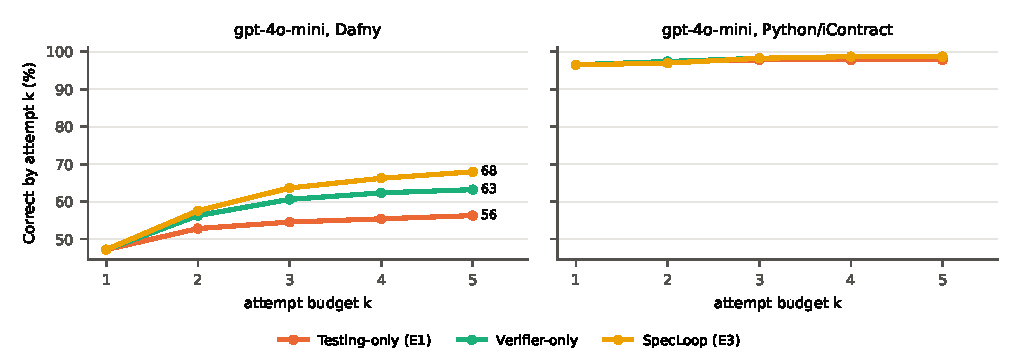
\includegraphics[width=\columnwidth]{generated/fig_curves.pdf}
\caption{Correctness after $k$ candidates (from per-candidate oracle verdicts). All configurations share the first candidate, so they start from the same point at $k=1$.}
\label{fig:curves}
\end{figure}

\textbf{Efficiency (E6).} On Dafny a run costs \R{dafny.single_shot.costrun}~m\$ (thousandths of a dollar) for single-shot generation, \R{dafny.testing_only.costrun}~m\$ for testing-only, \R{dafny.verifier_only.costrun}~m\$ for verifier-only and \R{dafny.specloop_full.costrun}~m\$ for SpecLoop, with \R{dafny.single_shot.calls}, \R{dafny.testing_only.calls}, \R{dafny.verifier_only.calls} and \R{dafny.specloop_full.calls} model calls per run on average. The cost that matters, though, is the cost per correct program. There, SpecLoop (\R{dafny.specloop_full.costsolved}~m\$) is cheaper than the verifier-only agent (\R{dafny.verifier_only.costsolved}~m\$), because the router lets it solve more tasks with slightly fewer calls. The testing-only agent is cheaper still per solved task (\R{dafny.testing_only.costsolved}~m\$), but it reaches a lower ceiling and, as shown above, cannot tell when its answer is unverified. Verification dominates the latency of the verifier-based loops: tool time is \R{rel.specloop_full.toolshare}\% of SpecLoop's model-plus-tool time, against \R{rel.testing_only.toolshare}\% for testing-only. On Python every configuration costs about the same, since nearly all runs end after one candidate. The whole study, including development runs and E2, cost \R{total.allspend}~USD in API calls.


\textbf{Reliability and the integrity guard (E6).} To test whether ``verified'' can be trusted, we built tampered versions of every reference solution: a dropped or weakened \texttt{ensures}, an added \texttt{requires false}, \texttt{assume false}, \texttt{\{:verify false\}}, an axiom lemma, an edited helper predicate, a removed or weakened iContract decorator, an added \texttt{require(lambda \ldots: False)}, a CrossHair-off comment, and a patched \texttt{icontract}. We also built harmless variants that only reformat or add comments. The guard rejected all \R{guard.dafny.tamper.n} Dafny and all \R{guard.python.tamper.n} Python tampering mutants and none of the \R{guard.dafny.benign.n} plus \R{guard.python.benign.n} harmless ones. Without the guard the result would have looked very different: Dafny alone accepted \R{guard.dafny.tamper.veraccepts} of the \R{guard.dafny.tamper.n} tampered programs, and CrossHair accepted \R{guard.python.tamper.veraccepts} of the \R{guard.python.tamper.checked} Python mutants we ran through it. In the actual runs GPT-4o-mini rarely tried to change the specification (the in-loop guard fired in \R{rel.specloop_full.runswithguardblock} SpecLoop run), so the guard is mostly insurance, but it is what lets us report a verified program as correct. The stagnation monitor switched to a rewrite in \R{rel.specloop_full.runswithswitch} SpecLoop runs, and \R{rel.specloop_full.solvedafterswitch} of those ended correct.
